
\section{Introduction}

The rapid progress of Large Language Models (LLMs) has markedly boosted artificial intelligence and machine learning due to their strong contextual text generation capabilities.
\feijie{Despite these groundbreaking advancements, recent works~\cite{EvaluationSurvey, wang2023evaluating} have highlighted the significance of LLMs evaluation.}
\cz{LLMs are prone to producing seemingly authentic yet factually inaccurate responses, a phenomenon known as hallucination~\cite{wang2023survey}. Such errors may stem from outdated or incorrect data during training or the model's learned associations, impacting its reliability.}
\feijie{The evaluation, therefore, helps identify instances of hallucination and understand the LLM's ability to generate coherent and contextually relevant text, i.e., factuality of LLM outputs.}




Recent efforts have been put into the factuality evaluation of LLM. For example, \cite{chen2023felm} introduce FELM, a benchmark comprising diverse factual samples across various domains. Moreover, \cite{tian2023finetuning} and \cite{feng-etal-2023-factkb} utilize external tools (e.g., search engines and a well-trained factual LLM) to estimate the factuality of the generated texts. Representing structured knowledge related to real-world objects, Knowledge Graphs (KGs) \cite{auer2007dbpedia, bollacker2008freebase, suchanek2007yago, carlson2010toward} have gained prominence for LLM factuality assessments. They primarily originate from Wikipedia, encapsulate factual information for AI tasks, and form the knowledge base with datasets like Natural Questions \cite{NaturalQuestions}. 


\pagebreak
Several studies \cite{sun2023head,liang2023holistic} have focused on creating benchmarks from knowledge sources by posing factual questions derived from triples in \cz{KGs}. %
These methods, as depicted in the left part of Figure \ref{fig:intro_demo}, either (i) sample subgraphs from large KGs or (ii) extract a subset of knowledge from text documents to construct multiple-choice or text question-answer pairs. Those question pairs are then posed to LLMs to assess their factuality.
However, the above-mentioned methods or evaluation strategies face challenges in comprehensively evaluating the factuality of LLMs. 
{\it Firstly}, \cz{the scope of evaluation data is often limited or incomplete, focusing predominantly on specific domains.}
\cz{This limitation restricts the evaluation's breadth and undermines its applicability across various contexts, failing to cover the wide range of topics LLMs are expected to handle.}
The specialized nature of these datasets means that the evaluation may not accurately reflect the model's performance in generating factual content across a broader spectrum of subjects. {\it Secondly}, the process of factuality evaluation itself is inherently time-consuming and costly. It necessitates that an LLM generate full texts, which must then be meticulously assessed for accuracy and reliability. 
\cz{This comprehensive generation and detailed review demand significant computational resources and extensive human effort~\cite{wang2023evaluating} for validation.}
As a result, the process becomes less feasible for regular or large-scale applications, limiting the frequency and scope of 
\cz{practical evaluations}.
{\it Lastly}, due to the limited size of the evaluation data, there may be biases in the benchmarks~\cite{gallegos2023bias}, or risks of test data leakage \cite{zhou2023dont}, which might compromise the validity of the evaluations.
Together, these challenges underscore the need for more scalable, efficient, and domain-agnostic approaches to evaluating the factuality of LLM-generated texts.




To this end, we propose \GraphEval{}, which consists of two novel features in terms of the design, as presented on the right side of Figure \ref{fig:intro_demo}. First, we utilize \cz{KGs} that encapsulate factual information sourced from verifiable content like Wikipedia. With the KG, millions of prompts can be automatically generated, leading to a significant saving of human efforts in labeling the ground truth. From the data perspective, the KG gives a more diversified and comprehensive evaluation of the LLMs' factuality. Second, the proposed method efficiently reduces the computation costs and speeds up the evaluation process. Specifically, we incorporate a highly reliable and lightweight judge model to decide whether an LLM can generate an accurate response to a designated question. 
Instead of generating the full text, the judge model returns three options (i.e., True, False, and I don't know) to simulate LLMs' responses to a given prompt. To ensure the reliability of the simulated results, the judge model is trained based on a few question-answer pairs, where the questions are sampled from KGs and the answers are generated by the target LLM. As a result, the judge model can serve as a replacement for the factuality evaluation of the facts extracted from large-scale KGs.   In summary, our contributions are as follows:



  

\begin{figure}[t]
    \centering 
    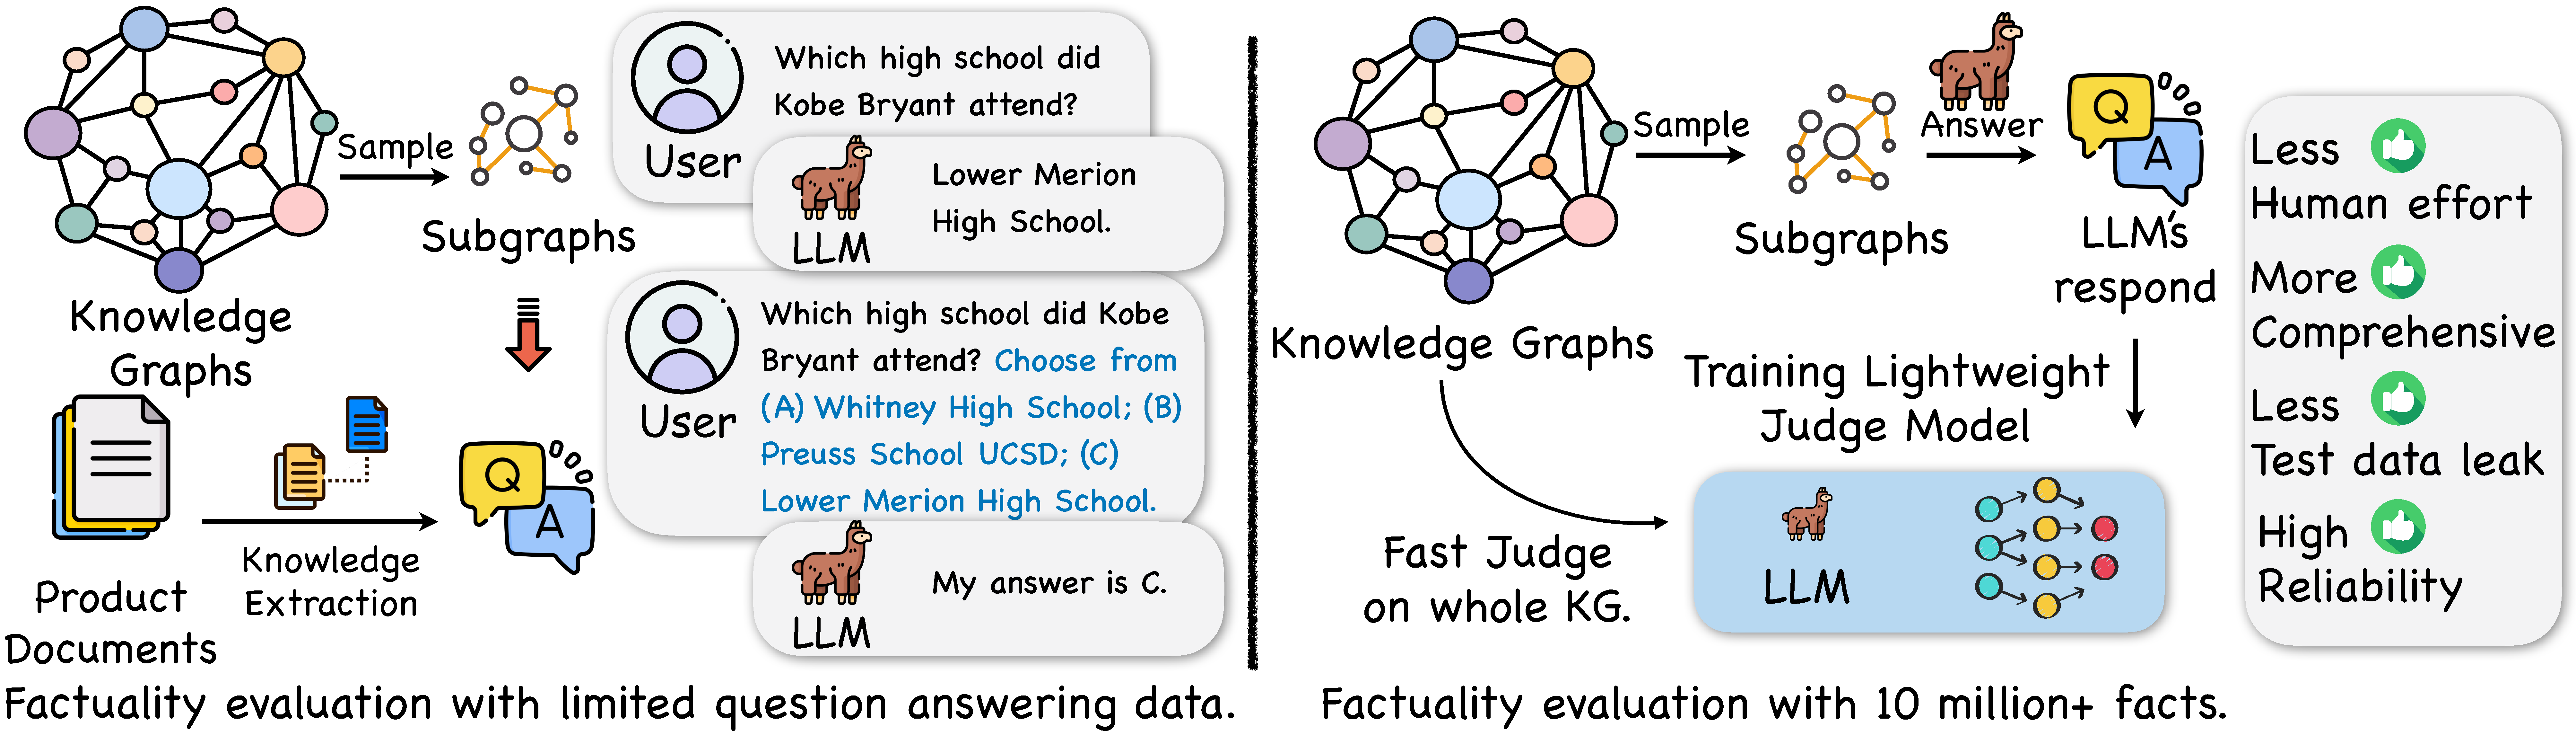
\includegraphics[width=.97\textwidth] {submissions/Jing2024/figures/intro_example.pdf} 
    \vspace{-2mm} 
    \caption{\feijie{Existing works compared to the proposed \GraphEval{} on factuality evaluation.}} 
    \vspace{-4mm}
    \label{fig:intro_demo}
\end{figure}  

\begin{itemize}[topsep=0pt,itemsep=0pt,parsep=0pt,partopsep=0pt,leftmargin=*]
    \item We propose \GraphEval{}, a large-scale evaluation framework that assesses the factuality of LLMs using KGs. \GraphEval{} evaluates the factuality of LLMs using the entire KGs, providing a more diversified and comprehensive evaluation of the LLMs' factuality.
    \item We introduce a judge model to assist with the evaluation process, which reduces the computational cost and enhances the efficiency of the evaluation. We also give a theoretical analysis of the judge model to demonstrate its validity.
    \item We conduct extensive experiments on a large-scale KG, i.e., DBpedia, to demonstrate the effectiveness and efficiency of \GraphEval{} in evaluating the factuality of LLMs.
    \item We provide an in-depth analysis of the LLM's performance on the KGs, including the LLM's performance with respect to relation types, head entity types, tail entity types, and the relation of LLM performance to degree and pageviews. 
\end{itemize}
     
